\chapter{Conception}

\section{Introduction}
This chapter converts the theoretical understanding of the domain into a concrete design for MapIT. The goal is to define what the system must do, how it should be organized, and which constraints guide the technical choices. The conception phase therefore bridges the gap between the problem statement and the formal modeling of the solution.

\section{Requirement Elicitation}
The expected needs of the platform were identified by examining the everyday tasks performed in documentation and incident-oriented IT workflows. This includes the need to consult knowledge quickly, register incidents with enough detail to be useful later, and keep the interface simple enough for non-specialists to use. The requirements were then separated into functional needs, which describe what the system must do, and non-functional needs, which describe how well it must do it.

\section{Functional Requirements}
The main functional requirements of MapIT are straightforward: users must authenticate securely, consult a dashboard, register incidents, create and update documentation entries, search content, and perform actions according to their role. Administrators must be able to manage sensitive operations, while standard users should still have access to the knowledge base and incident records required for their work. This definition keeps the first release focused on core operational value rather than peripheral features.

\section{Non-Functional Requirements}
Several non-functional qualities are important for this type of system. Security is necessary because the platform stores operational information and controls access to it; usability matters because the knowledge base must be easy to navigate under time pressure; maintainability is important because the application should remain understandable as it evolves; and traceability is needed so that users can trust the history of the data. Performance and reliability also matter, even in an academic prototype, because slow search or unstable access would immediately reduce adoption.

\section{High-Level Architecture}
MapIT follows a simple three-tier architecture composed of a frontend, a backend API, and a relational database. The frontend is responsible for the user experience, the backend handles business logic and authorization, and the database stores the structured records that support incidents, documents, and users. This separation improves maintainability and makes the system easier to evolve because each layer has a clear responsibility.

Figure~\ref{fig:architecture-mapit} presents the concrete architecture used in the project, including the web client, API server, and persistence layer.

\begin{figure}[H]

	\centering
	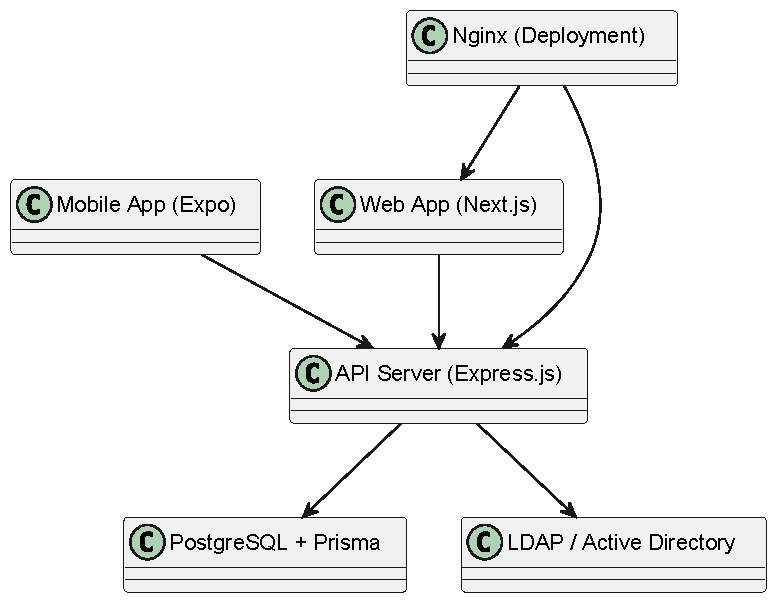
\includegraphics[width=0.95\textwidth]{figures/diagrams/architecture_diagram.pdf}
	\caption{High-level architecture of MapIT}
	\label{fig:architecture-mapit}
\end{figure}


\section{Module Decomposition and User Journeys}
The system is divided into modules that reflect the main business activities of the platform: authentication, dashboard visualization, incident management, document management, and administration. A typical user journey begins at login, continues with a dashboard overview, and then leads to either the creation of a new record or the consultation of an existing one. This modular design keeps the application understandable and allows each user role to follow a path that matches its responsibilities.

\section{Design Decisions and Constraints}
The design choices are driven by a need for data consistency, controlled access, and easy navigation. A centralized data model avoids duplication between incidents and documents, while role-based rules prevent unauthorized modification of critical records. At the same time, the interface must remain clean and direct so that the system can be used as a practical knowledge tool rather than as a purely theoretical database.

\section{Chapter Conclusion}
The conception phase establishes a clear functional direction for the application and frames the main constraints that the implementation must respect. It shows that MapIT is intentionally focused on the workflows that matter most for incident-oriented documentation. The next chapter formalizes this design through UML and data modeling artifacts.
